\section{Process' Perspective}
\label{process-perspective}

\subsection{Communication between developers}

The communication between team members was equally conveyed through both physical and remote working sessions. We worked and communicated to a large extent on the days when the course lectures were given. Furthermore, the use of Microsoft Teams allowed us to work and communicate remotely whenever it was needed. Each week the team were updated on tasks that were not finished from previous weeks and planned prioritization of said tasks based on the state of the system. If anyone had a question or a concern, a team member could ask in the Teams chat and resolve the problem rather quickly.  

\subsection{Team organization}

Everyone in the team had the same responsibilities and roles in the team. We focused on including every group member in the development process, such that everyone was up to date. We would provide and go through an agenda for the day we were working, where the agendas were based on the state of the project and the latest lecture. 

Furthermore, the team was composed of people with varying experiences with DevOps ranging from zero to professional experience prior to starting the course. This meant that we had to get everyone on the same level during some sessions together to prevent some group members from falling behind on the course material. 

Finally, in relation to getting everyone in touch with most parts of the code and project, we did not enforce any strict rules about whom works on what, and we endorsed everyone to work on things that they would like to, such as a specific technology or language (Go, Docker, Vagrant etc.) to be able to take ownership of the application.


\subsection{Stages and tools in CI/CD chain}
We initially wanted to use Travis CI for our CI/CD chain. Unfortunately, Travis CI was out of the scope economically since they changed their policy recently related to their pricing model. Therefore, we resorted to GitHub Actions instead. We used GitHub Actions to automate our integration and release pipeline. We have three GitHub action workflows: 
\begin{itemize}
    \item \textit{Continuous Integration}: The integration workflow is running some static code-checks\footnote{See: \url{https://github.com/ITU-DevOps-N/go-minitwit/blob/develop/.github/workflows/continuous-integration.yml} for a list of services used} and tries building the Golang. application.
    \item \textit{Continuous Deployment}: The deployment workflow will build Docker images for both the API and the application and push them to Docker Hub. After it will login into the machine, which is being hosted on DigitalOcean, and deploy the system.
    \item \textit{GitHub release}: Fetches the latest version of the application from an API endpoint and makes a new GitHub release automatically.
\end{itemize} 

A visual representation can be seen in Figure \ref{fig:cicd} found in appendix \ref{app:cicd}.





%A complete description of stages and tools included in the CI/CD chains.
%That is, including deployment and release of your systems.


%Organization of your repositor(ies).
    %That is, either the structure of of mono-repository or organization of artifacts across repositories.
    %In essence, it has to be be clear what is stored where and why.
\subsection{Repository organization}

At the top level of our repository, we have our configuration files (vagrantfile, Dockerfile, docker-compose, iac.sh, etc.), and other documentation files such as licenses, service level agreements, \texttt{README.md} and a bash script (wait\_for\_release.sh) that is used in the CD to wait for the new release version is deployed before starting the "GitHub release" GitHub Action workflow. The script iac.sh is used to create the infrastructure on DigitalOcean from scratch, it runs vagrant and then it connects to the machines to set up the Docker Swarm Cluster. To separate functionality we have organized folders in a way to isolate features: \texttt{src}, \texttt{monitoring}, \texttt{api} and \texttt{.github/workflows} are the most critical packages that are involved in our system. 
\begin{itemize}
    \item The \texttt{src} folder contains most of our codebase, containing structure and models for the database, test files, controllers, and static front-end layout files.
    \item The rest of the codebase is stored in \texttt{api}, where we keep our API for interacting with the user simulator.
    \item In \texttt{monitoring} we have our relevant monitoring files (Prometheus/Grafana).
    \item In \texttt{.github/workflows} we have the configuration files for Github Actions.
\end{itemize}

\subsection{Applied Branching Strategy}

\subsubsection*{Branching model}
\begin{itemize}
    \item \texttt{main}: Entirely stable code should reside here, possibly only code that has been or will be released. Code in this branch will go through the CI/CD pipeline.
    \item \texttt{develop}: A parallel branch that is worked from or used to test stability — it is not necessarily always stable, but whenever it gets to a stable state, it can be merged into main. Used to pull in topic branches, i.e. hotfixes, features etc. Tested on develop and merged into main.
    \item \texttt{feature/}: A short-lived branch that you create and use for a single particular feature or related work.
\end{itemize}

Whenever a group member wants to add code to the repository, the first step they do is to create a new branch, \texttt{feature/<feature\_name>}, where \texttt{<feature\_name>} is to be replaced with a descriptive name. Once the feature is ready, the developer will create a pull request from the \texttt{feature/<feature\_name>} branch to the \texttt{develop} branch. All the main functionalities of the system should work in the \texttt{feature/<feature\_name>} branch before approving the pull request. At least one reviewer will be required to approve the pull request. Once the pull request has been merged, the \texttt{feature/<feature\_name>} branch should be deleted locally and remotely. Once a stable release is made, the \texttt{develop} branch will be merged into the \texttt{main} branch. At least two reviewers will be required to approve the pull request. The process is illustrated in the figure below.
\begin{figure}[ht]
		\centering
		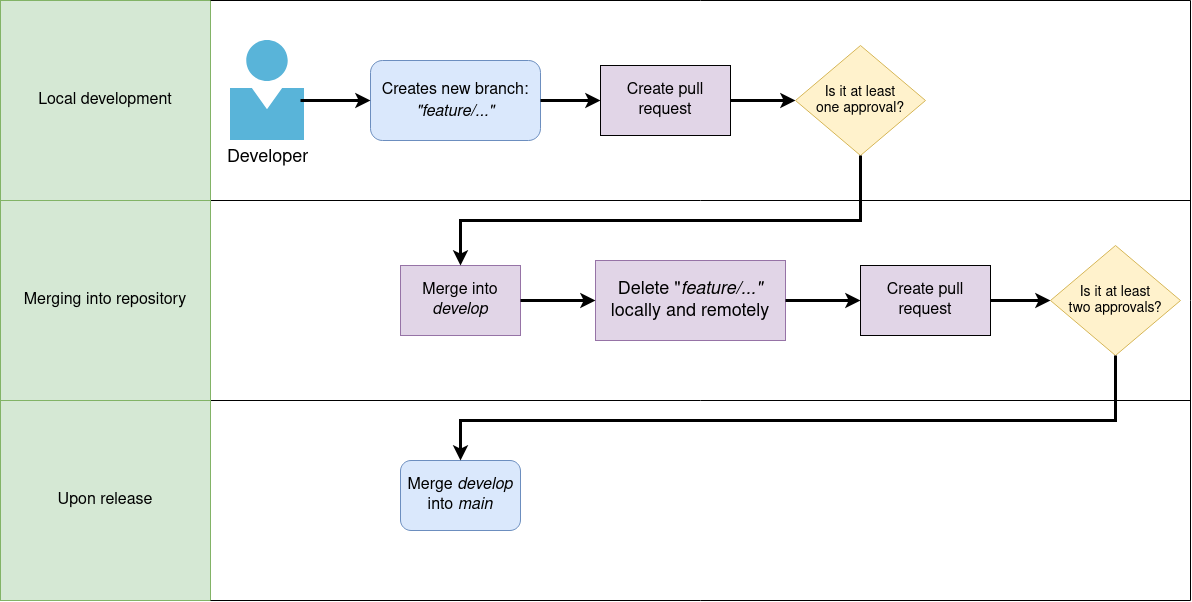
\includegraphics[width=\textwidth]{images/branching.drawio.png}
		\caption{Branching strategy}
		\label{fig:example}
\end{figure}


%For example, how did you use issues, Kanban boards, etc. to organize open tasks
\subsection{Applied Development Process and Tools Supporting It}
We used Github issues to declare new tasks that needed our attention. Whenever a group member encountered a problem that needed to be addressed, they would create a new issue describing what needs to be done. In addition to Github issues, we also configured Bugsnag to automatically create GitHub issues. If something was critical and needed to be done urgently, we made use of the "urgent message" function in Microsoft Teams, which notifies all members of a chat in time intervals until it is toggled off.

\subsection{How do you monitor your systems and what precisely do you monitor?}
For monitoring our system we are using Prometheus, an open-source monitoring system offering dimensional data models, flexible query language and a modern alerting approach. It collects and stores its metrics (numeric measurements) as time-series data, e.g. the metrics information gets stored along with a timestamp indicating at which time it was recorded, additionally with key-value pairs called labels. 

Prometheus is configured in \texttt{Prometheus.yml} 

We choose to monitor the following metrics of our system:
\begin{itemize}
    \item \textbf{CPU Load Percentage} - provides information about the processor (CPU) load, in percentage, of both the API and Web systems.  
    \item \textbf{Gin Total Requests} - shows the number of total requests on web-app and API
    \item \textbf{Prometheus Process Memory} - give information about the amount of memory the Prometheus process is using from the kernel
    \item \textbf{Go Memory Stats} - displays how much memory the go process is using at a certain time.
\end{itemize}

Then we use Grafana and its dashboard to analyze/visualize data queries from Prometheus, to give a nice monitoring overview of the system. See Grafana Dashboard at appendix \ref{app:grafanamonitoring}.

\subsection{What do you log in your systems and how do you aggregate logs?}
%Elk stack, filebeat, Kibana to aggregate, present , elasticsearch to filter, Response codes 200, 404 etc.

For logging, we use the \textit{ELK stack} to store, search, ingest and visualize data collected from our system, in addition to \textit{filebeat} to aggregate logs. Within our \texttt{filebeat.yml} we specify that we take input from all containers in our docker setup. The output filters the data to the index which contains logs in form of response codes from our \textit{ITUMiniTwit} application, including messages that contain the keywords "\texttt{ERR}", "\texttt{WARN}" and "\texttt{GIN}". The configuration for our logging output can be seen in the figure below.
\begin{figure}[ht]
    \centering
    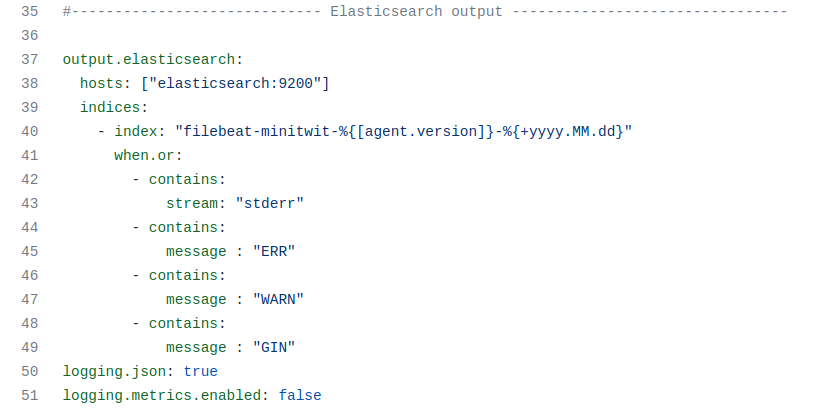
\includegraphics[width=0.9\textwidth]{images/filebeat-snippet.png}
    \caption{Snippet from \texttt{filebeat.yml}}
    \label{fig:filebeat}
\end{figure}

Finally, we use Kibana to visualize the filtered data to dashboards, where the data can be analyzed into for example graphs, charts and heatmaps.

\subsection{Brief results of the security assessment}
We used Arachni to  do a penetration test of our API, which showed that we have some issues with cross-site-forgery, unencrypted password forms, common directories, password fields with auto-complete, and missing X-frame Options header\footnote{Some of these issues were fixed}. However, these issues were either reported once or twice during a 24 hours penetration testing and the other group who were penetrating testing our API were not able to find any vulnerabilities.  \footnote{See full Risk identification and analysis here \cite{security} and pen-test report here \cite{pen-test}}


\subsection{Applied strategy for scaling and load balancing}

\textbf{Scaling:} we can summarize the scaling strategies into Vertical and Horizontal Scaling. 
\begin{itemize}
    \item \textbf{Vertical scaling} - we resized the virtual machines into DigitalOcean, increasing the CPU and RAM of these latter. This was the solution that was chosen instead of increasing the number of machines because of cost convenience.
    \item \textbf{Horizontal scaling} -  Docker Swarm cluster makes it possible to scale our containers horizontally. This can be achieved either through manual maintenance or editing the docker-compose file.
\end{itemize}

Both of them were not automated and therefore human interaction was required in order to perform scaling of any kind. If we observed that one or more of the virtual machines that were hosted on DigitalOcean had too much load on for example CPU or memory usage, we would perform vertical scaling to the existing machines by upgrading their specs or horizontally by increasing the number of containers.

\textbf{Load Balancing: }currently there are three virtual machines hosted on DigitalOcean and they are all part of the Docker Swarm cluster, one manager and two worker nodes. All the containers are spread among these machines. Our main endpoint is exposed by DuckDNS and it points to the manager node's IP. Every time a service is called through this endpoint, it is resolved by Docker Swarm, no matter in which node the service's container is located.

%In essence it has to be clear how code or other artifacts come from idea into the running system and everything that happens on the way.